%\documentclass[draft]{beamer}
\documentclass{beamer}
\usetheme{Warsaw}
\usecolortheme{wolverine}
\usepackage{graphicx}
\usepackage{amsmath}
\usepackage{amsfonts}
\usepackage{amssymb}
\usepackage{amsthm}
\DeclareMathOperator{\Li}{Li}

\title[Prime Numbers]{Prime Numbers and the Riemann Hypothesis}
\subtitle{(Writing a book with Barry Mazur)}
\author[W.\thinspace{}Stein]{William Stein}
\date[Mazur 80]{June 4, 2018 at Harvard University}
\institute[SageMath, Inc. \& UW]{SageMath, Inc. and University of Washington}

\begin{document}

\begin{frame}
  \titlepage
\end{frame}

\begin{frame}{Abstract}
  \begin{abstract}
    In 2004, Barry Mazur and I started writing the
    book ``Prime Numbers and the Riemann Hypothesis'', which we recently
    published with Cambridge University Press. I'll talk about
    what's in the book and why, describe some of the technical aspects
    of production of the book, and tradeoffs for us between
    self publishing online versus with a traditional publisher.

    \vspace{.3in}
    This is talk about talking about the Riemann Hypothesis.
  \end{abstract}
\end{frame}

\begin{frame}{Overview}
  \tableofcontents
\end{frame}

\begin{frame}{The book...}
  \begin{center}
    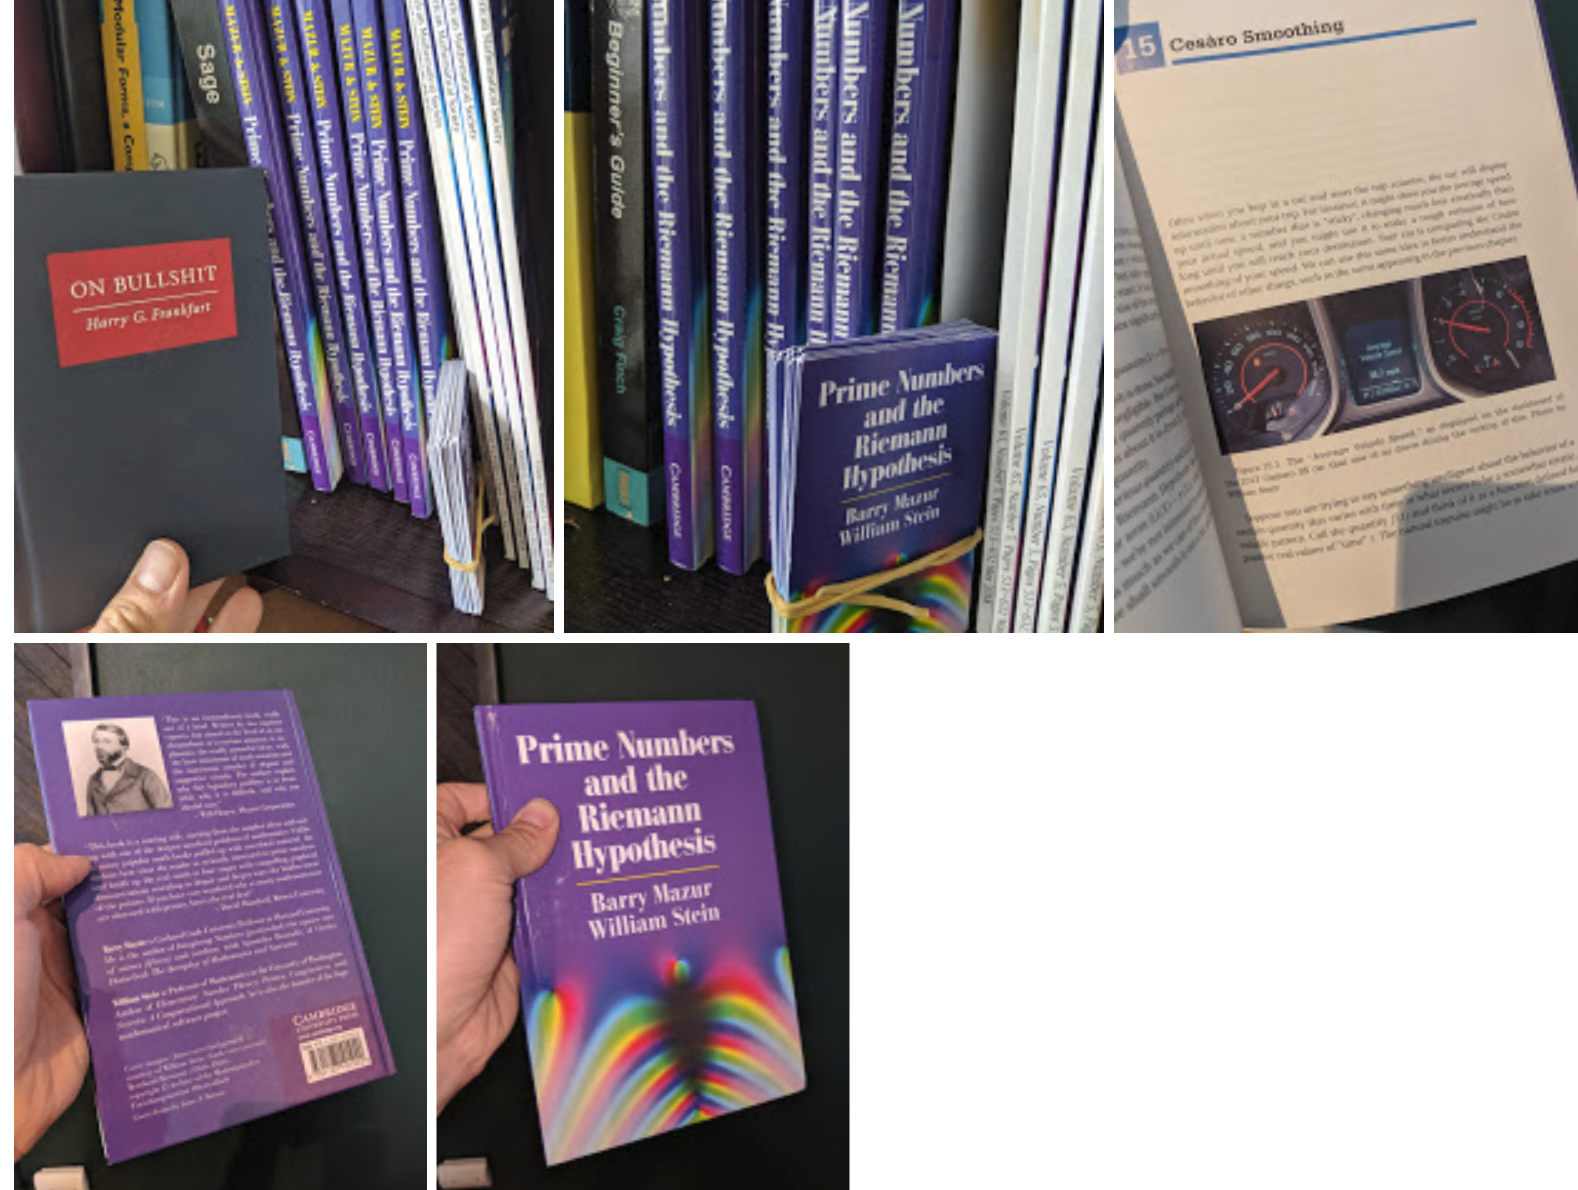
\includegraphics[height=.82\textheight]{pics/the-book.png}
  \end{center}
\end{frame}

\section{A Public Lecture}

\begin{frame}{Clay Math Institute public lecture (MIT, May 3, 2005)}

  \href{http://www.claymath.org/library/public\_lectures/mazur\_riemann\_hypothesis.pdf}{\bf Are there still unsolved problems about the numbers 1, 2, 3, 4, ... ?}
  \vfill

  \begin{block}{``Sell'' number theory to the general public}
    \begin{itemize}
      \item   Immediately accessible
      \item   Immediately interesting
      \item   Primes and how eratic they are
      \item   Cicada's every 13, 17 years...
      \item   Lots of examples that are ``opening, interesting questions/issues.''
      \item   People can immediately make computations of their \underline{own}
      \item   Barry Mazur got his father who had done NO
            math hooked on Goldbach Conjecture, so thought
            primes would work.
    \end{itemize}
  \end{block}
\end{frame}

\begin{frame}{SageMath}
  \vfill
  \begin{center}
    
\includegraphics[width=.7\textwidth]{pics/sage-logo.png}
  \end{center}
  \vfill

  \begin{block}{I started SageMath}
    I launched Sage a few months before this 2005 CMI public lecture.
    \begin{itemize}
      \item Sage is a free open source alternative to Mathematica, Maple, Magma, and Matlab.
      \item Early Sage development was motivated by this talk
            \begin{itemize}
              \item Linking Sage to Mathematica to compute the incomplete Gamma function.
              \item Early plotting functionality.
            \end{itemize}
    \end{itemize}
  \end{block}
\end{frame}

\begin{frame}{More about what was in the public lecture...}

\end{frame}


\section{Write a Book}

\begin{frame}{Let's write a book...}
  \begin{block}{Turn this lecture into a book.}

    \begin{itemize}
      \item Write something for a popular audience.
      \item Small and readable.
      \item Full of {\em mathematics}, not stories of people.
      \item Profusely illustrated.
      \item Meet for a few weeks each year and focus on this.
    \end{itemize}
  \end{block}
\end{frame}

\begin{frame}{The Prime Counting Problem}
  Let $\pi(x)$ be the number of primes $\leq x$.\\
  Problem: give a ``good approximation'' for $\pi(x)$.
  \vfill

  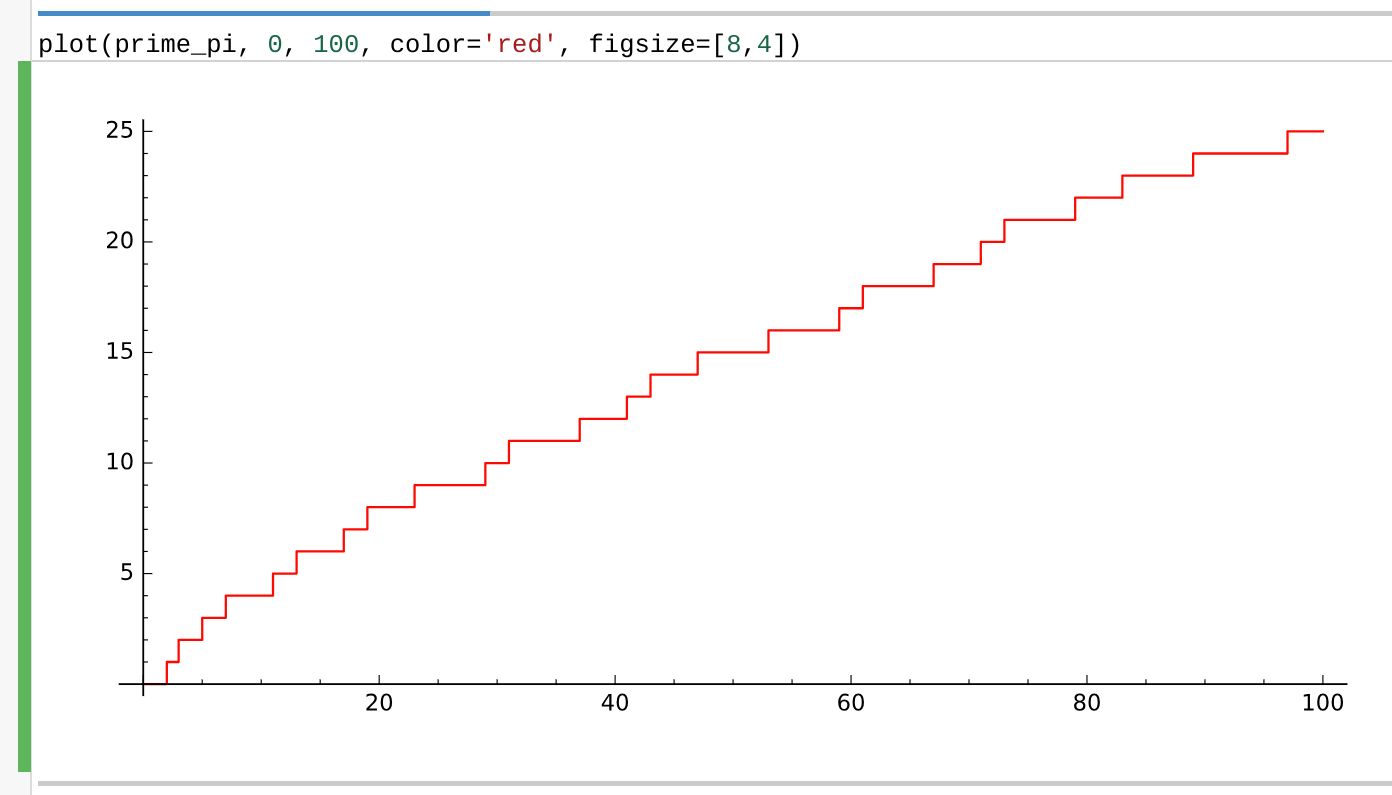
\includegraphics[width=.98\textwidth]{pics/prime-pi-100.png}

\end{frame}

\begin{frame}{The Prime Counting Problem}
  Let $\pi(x)$ be the number of primes $\leq x$.\\
  Problem: give a ``good approximation'' for $\pi(x)$.
  \vfill

  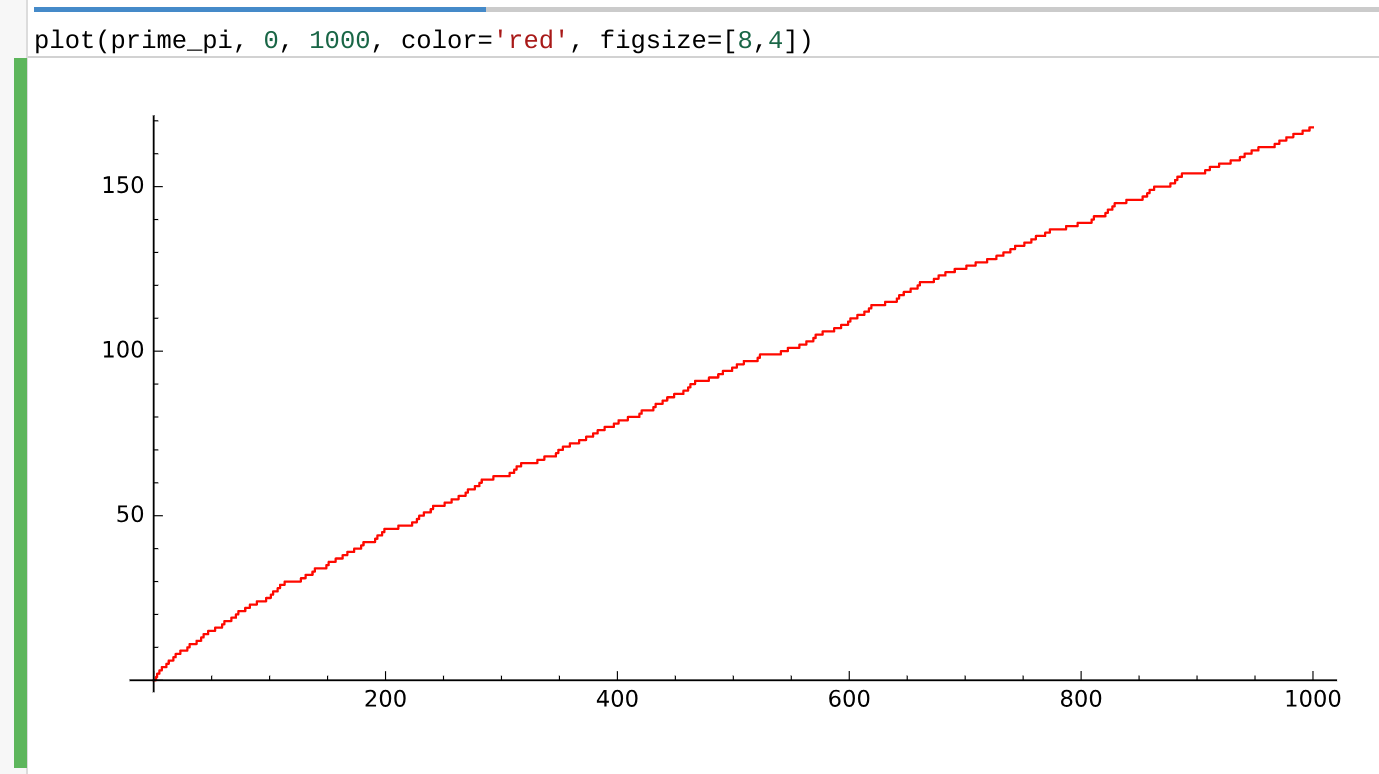
\includegraphics[width=.98\textwidth]{pics/prime-pi-1000.png}

\end{frame}

\begin{frame}{The Prime Counting Problem}
  Let $\pi(x)$ be the number of primes $\leq x$.\\
  Problem: give a ``good approximation'' for $\pi(x)$.
  \vfill

  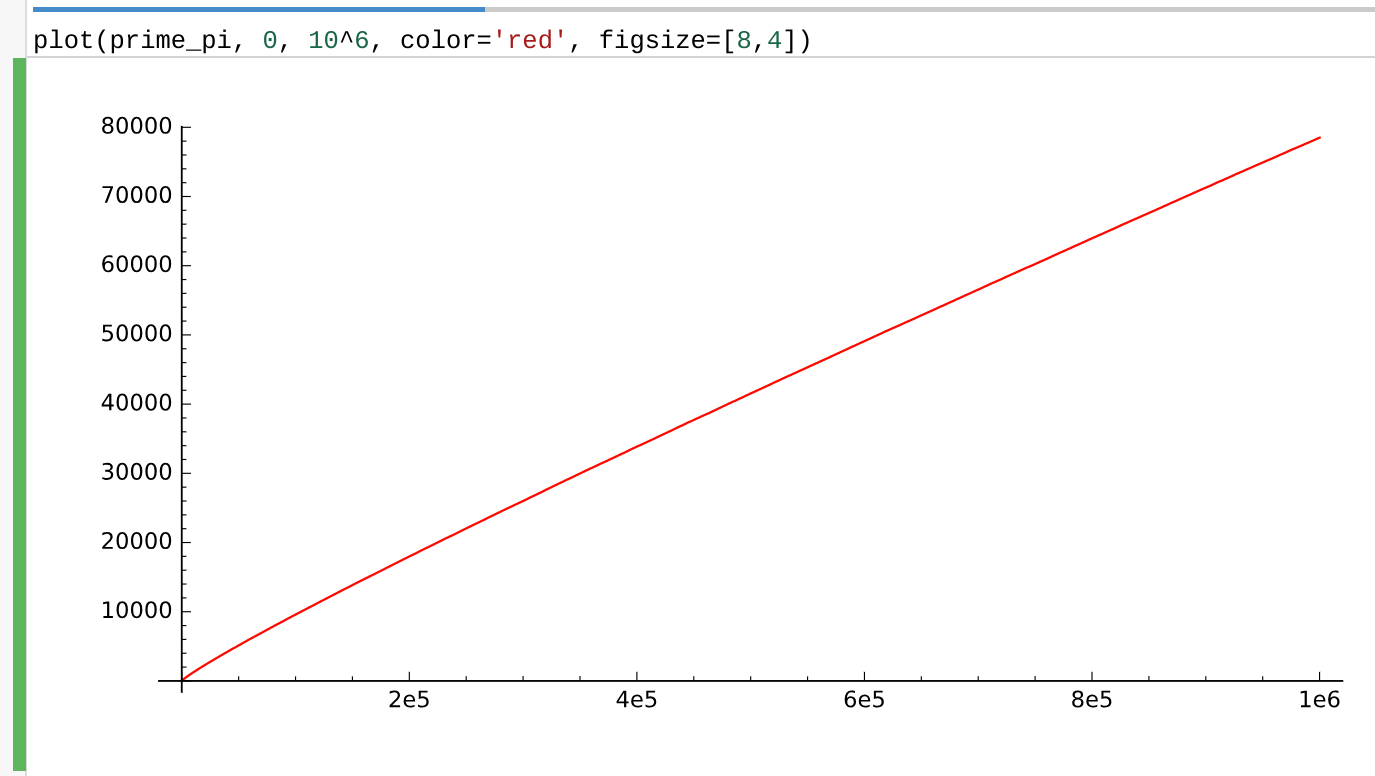
\includegraphics[width=.98\textwidth]{pics/prime-pi-1000000.png}

\end{frame}

\begin{frame}{Answer: The Riemmann Hypothesis (first formulation)}
  \begin{block}{}
    The number of prime numbers less than $X$ is
    approximately $\Li(X)$ and this approximation is essentially square
    root accurate.
  \end{block}
  \begin{center}
    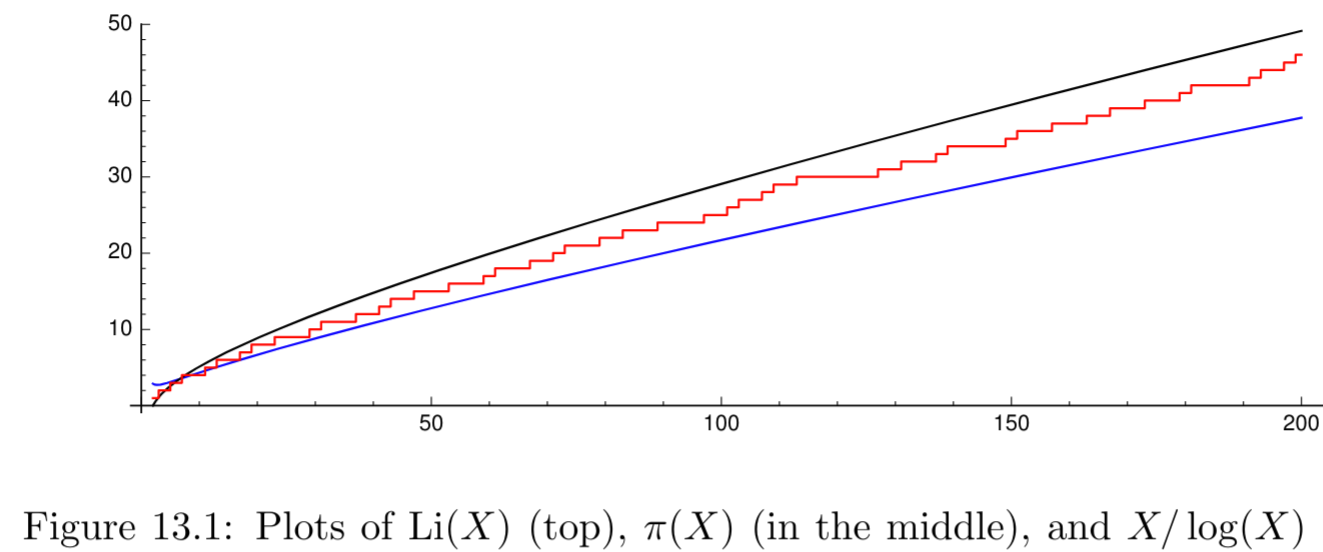
\includegraphics[width=.5\textwidth]{pics/plot-pi-Li.png}
    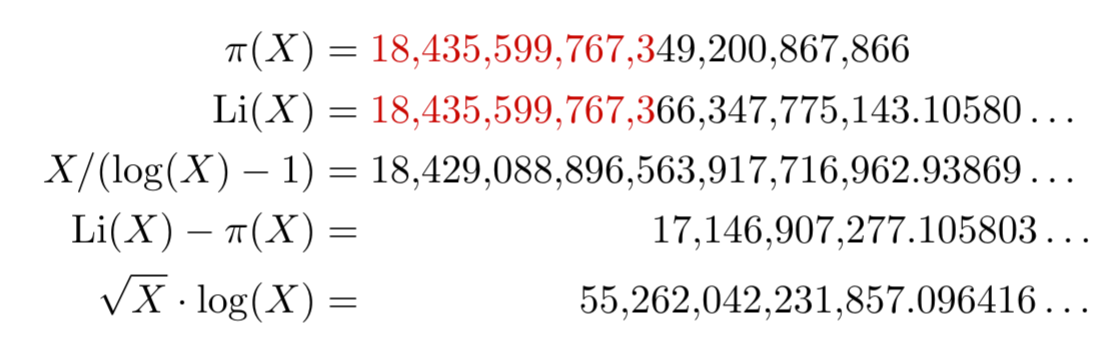
\includegraphics[width=.5\textwidth]{pics/ten24.png}
  \end{center}
\end{frame}

\begin{frame}{Answer: The Riemmann Hypothesis  (second formulation)}
  \begin{block}{}
    The prime power staircase $\psi(X)$ is essentially square root close
    to the 45 degree straight line.
  \end{block}

  $\psi(x)$: Our staircase starts on the ground at $x=0$ and the height of the
  riser of the step at $x=1$ will be $\log(2\pi)$. The height of the
  riser of the step at $x=p^n$ will not be $1$
  but rather: the step at $x=p^n$ will have the height of its riser
  equal to $\log p$.


\end{frame}

\begin{frame}{Answer: The Riemmann Hypothesis (third formulation)}
  \begin{block}{}
    Basically, \textit{the explicit formula}: the Fourier transform
    of the derivative of $\psi(X)$ ``is'' a discrete distribution (supported
    at the real parts of the zeros of the Riemann Zeta function).
    We deleted this from book, since it was too technical
    to precisely state.  .)
  \end{block}

  (illustrative plot.)


\end{frame}



\begin{frame}{Answer: The Riemmann Hypothesis (fourth formulation)}
  \begin{block}{}
    All the nontrivial zeroes\index{nontrivial zeroes} of $\zeta(s)$ lie on the vertical
    line in the complex plane consisting of the
    complex numbers with real part equal to $1/2$.
  \end{block}
\end{frame}


\begin{frame}{What kind of book?}
  \begin{itemize}
    \item   Book motivated by the prime counting problem (connect with other project -- explicit formula projects...).
    \item Mostly math and no ``stories of people'', since many other books on RH do that already.
    \item Similar problem to guessing rank of an elliptic curve from $a_p$, which we had been thinking about.
  \end{itemize}
\end{frame}

\begin{frame}{What Sort of Book?  Big? Small?}
  \begin{center}
    Like T.\thinspace{}C. MITS or like ON BULLSHIT?
    \vspace{1ex}

    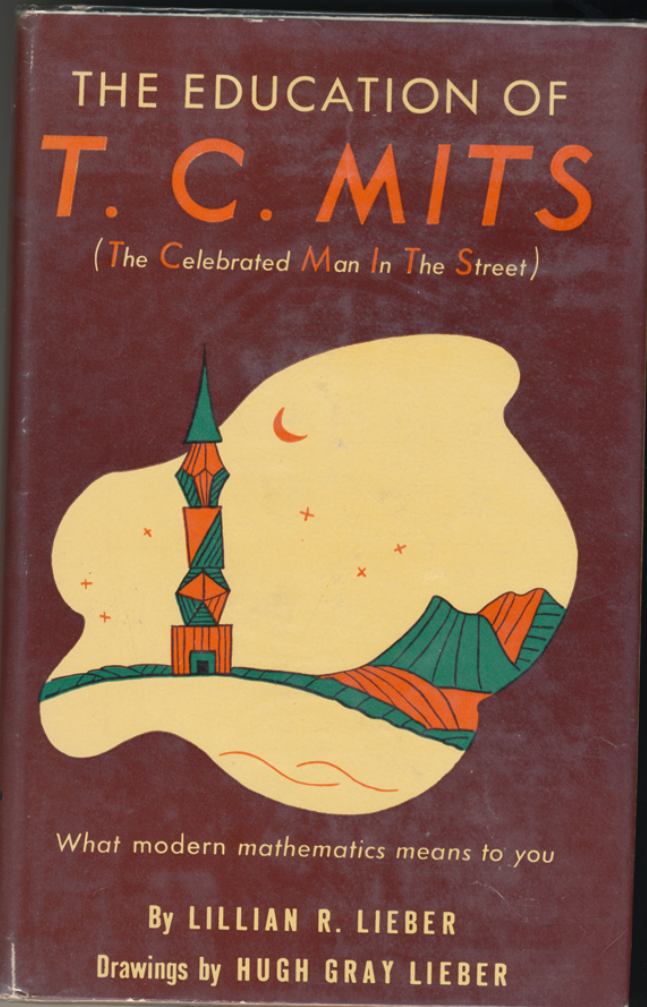
\includegraphics[height=.75\textheight]{pics/tc-mits.png}
    \hspace{2em}
    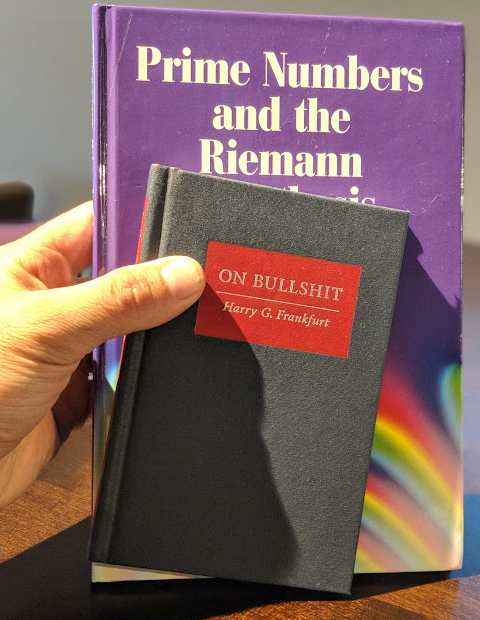
\includegraphics[height=.75\textheight]{pics/bullshit.png}
  \end{center}
\end{frame}


\begin{frame}{Our Approach}
  \begin{block}{}
    \begin{itemize}
      \item Do not emphasize people/history/stories, since that's done already in many other books on RH.
      \item   Go back 150+ years and explain what RH is more from the point of view of real classical Fourier analysis.
            \begin{itemize}
              \item We embraced this mid-19th century real perspective.
              \item We left complex numbers to the very, very end.
            \end{itemize}
    \end{itemize}
  \end{block}
  \begin{center}
    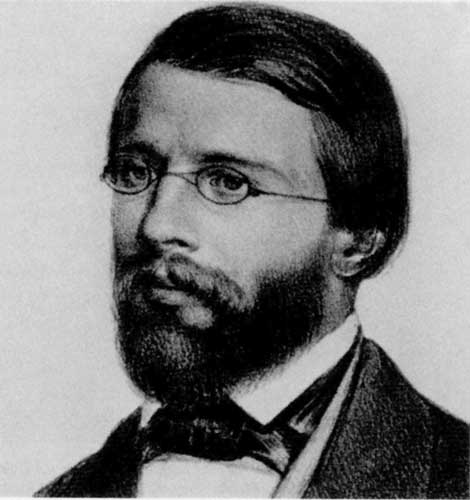
\includegraphics[height=.4\textheight]{pics/riemann}
  \end{center}

\end{frame}


\begin{frame}{Target Audience?}

  Who are we writing this book for? Those who want to read about mathematics (not people and history).

  \begin{itemize}
    \item \textbf{High School students?} Tested at \href{https://wstein.org/edu/2007/simuw07/}{SIMUW 2007}.
    \item \textbf{Retired electrical engineers?}  Tested with original MIT talk, and  online materials we shared.
  \end{itemize}


\end{frame}


\begin{frame}{SageMath again}
  Used Sage to compute with prime numbers, zeros, etc., and generally to plot everything in the book.
  \begin{itemize}
    \item We drew tons of plots to illustrate everything.
    \item The plots are absolutely essential to the exposition, and in fact really drove it!
    \item It is surprising that you see the spikes with such little computation.
    \item Central observations:
          \begin{itemize}
            \item Fourier transform of discrete distribution at primes, gives discrete distribution of zeros of $\zeta$.
            \item The reverse gets the discrete distribution of prime powers.
          \end{itemize}
    \item This what got us thinking about ``how explicit is the explicit formula if you compute?''
  \end{itemize}
\end{frame}


\begin{frame}{Collaborative \LaTeX{} via CoCalc}
  \begin{block}{}
    \begin{itemize}
      \item Using CoCalc's \LaTeX{} editor.
            \begin{itemize}
              \item Web browser...
              \item Gives a sense of the collaborative spirit
              \item Plug: a brand new version of this was just released.
            \end{itemize}
      \item We put a rough PDF of book on the web at every stage.
      \item GitHub: \url{https://github.com/williamstein/rh}
    \end{itemize}
  \end{block}
\end{frame}


\section{Publish a Book}

\begin{frame}{How to Publish the book:  Self publish!?}
  \begin{itemize}
    \item Self publishing: just put it on my website and see what happens.
          \begin{itemize}
            \item Enormous number of people that proof read it.
            \item Will Hearst pushed us for proper publication.
          \end{itemize}
  \end{itemize}
\end{frame}

\begin{frame}{Finding a commercial publisher}
  \begin{itemize}
    \item Finding a publisher
    \item What expected to give is \LaTeX{}...
  \end{itemize}
\end{frame}


\begin{frame}{Typos and Mistakes}
  \begin{itemize}
    \item Dozens of people carefully read drafts of
          the book and provided incredibly useful feedback.
          \textbf{THANK YOU!}
    \item The publisher also had a copy editor read the book,
          and provided complementary feedback.
    \item Don't expect your publisher to catch the sort of
          mistakes a mathematician catches:
          \begin{center}
            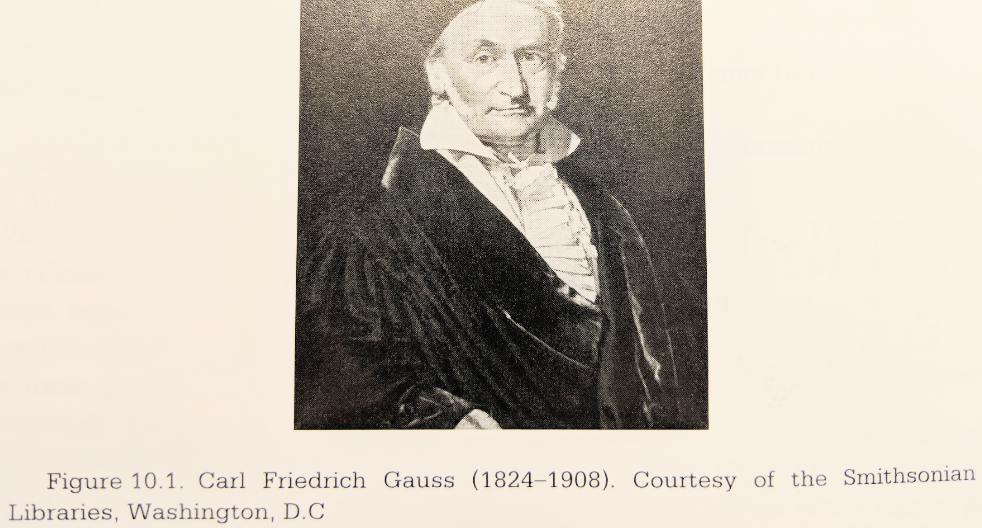
\includegraphics[height=.45\textheight]{pics/gauss.png}
          \end{center}
  \end{itemize}
\end{frame}


\begin{frame}{Creating a Cover}
  \begin{itemize}
    \item ...
  \end{itemize}
\end{frame}


\begin{frame}{Endorsements for the back cover}
  \begin{itemize}
    \item ...
  \end{itemize}
\end{frame}

\begin{frame}{Production}
  \begin{itemize}
    \item Cambridge Univ Press might have made some positive steps toward \LaTeX{} (mention Ogus).
    \item Working with CUP has been a very positive experience overall.
  \end{itemize}

\end{frame}

\begin{frame}{Published!}

  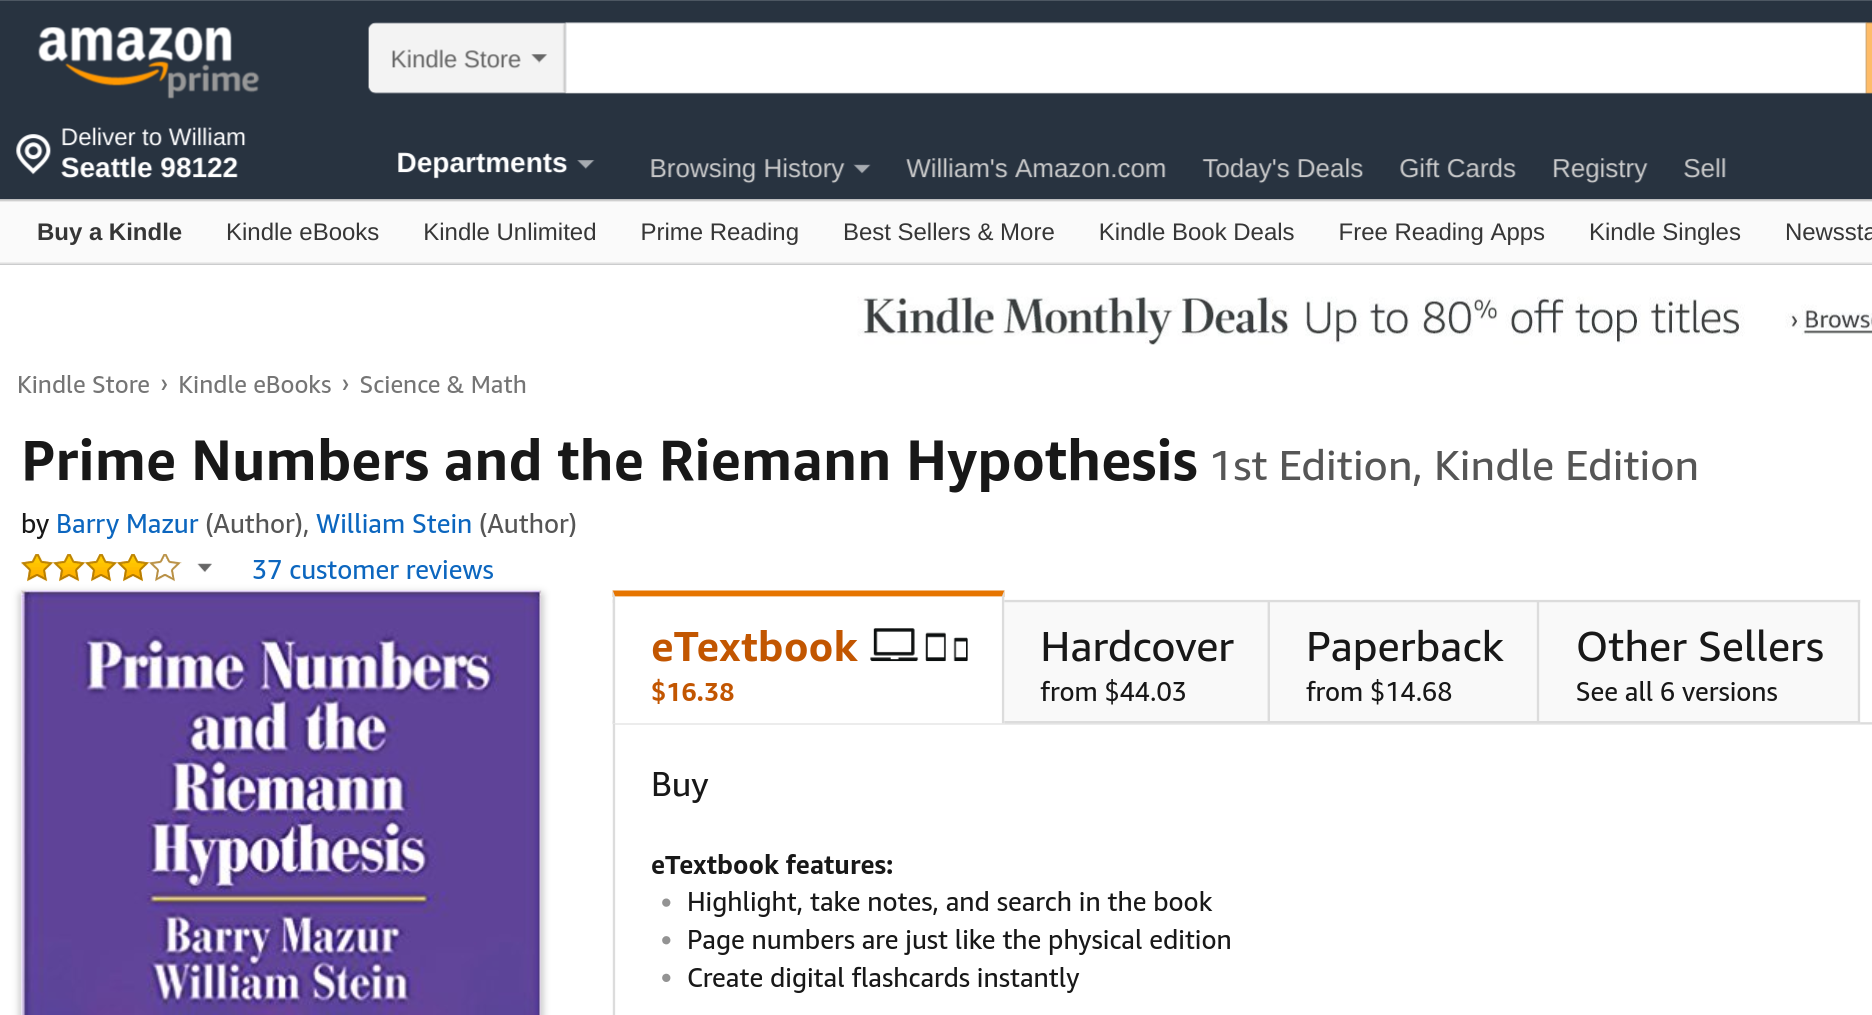
\includegraphics[width=.98\textwidth]{pics/amazon-prime.png}

\end{frame}



\begin{frame}{Reviews by Readers}

  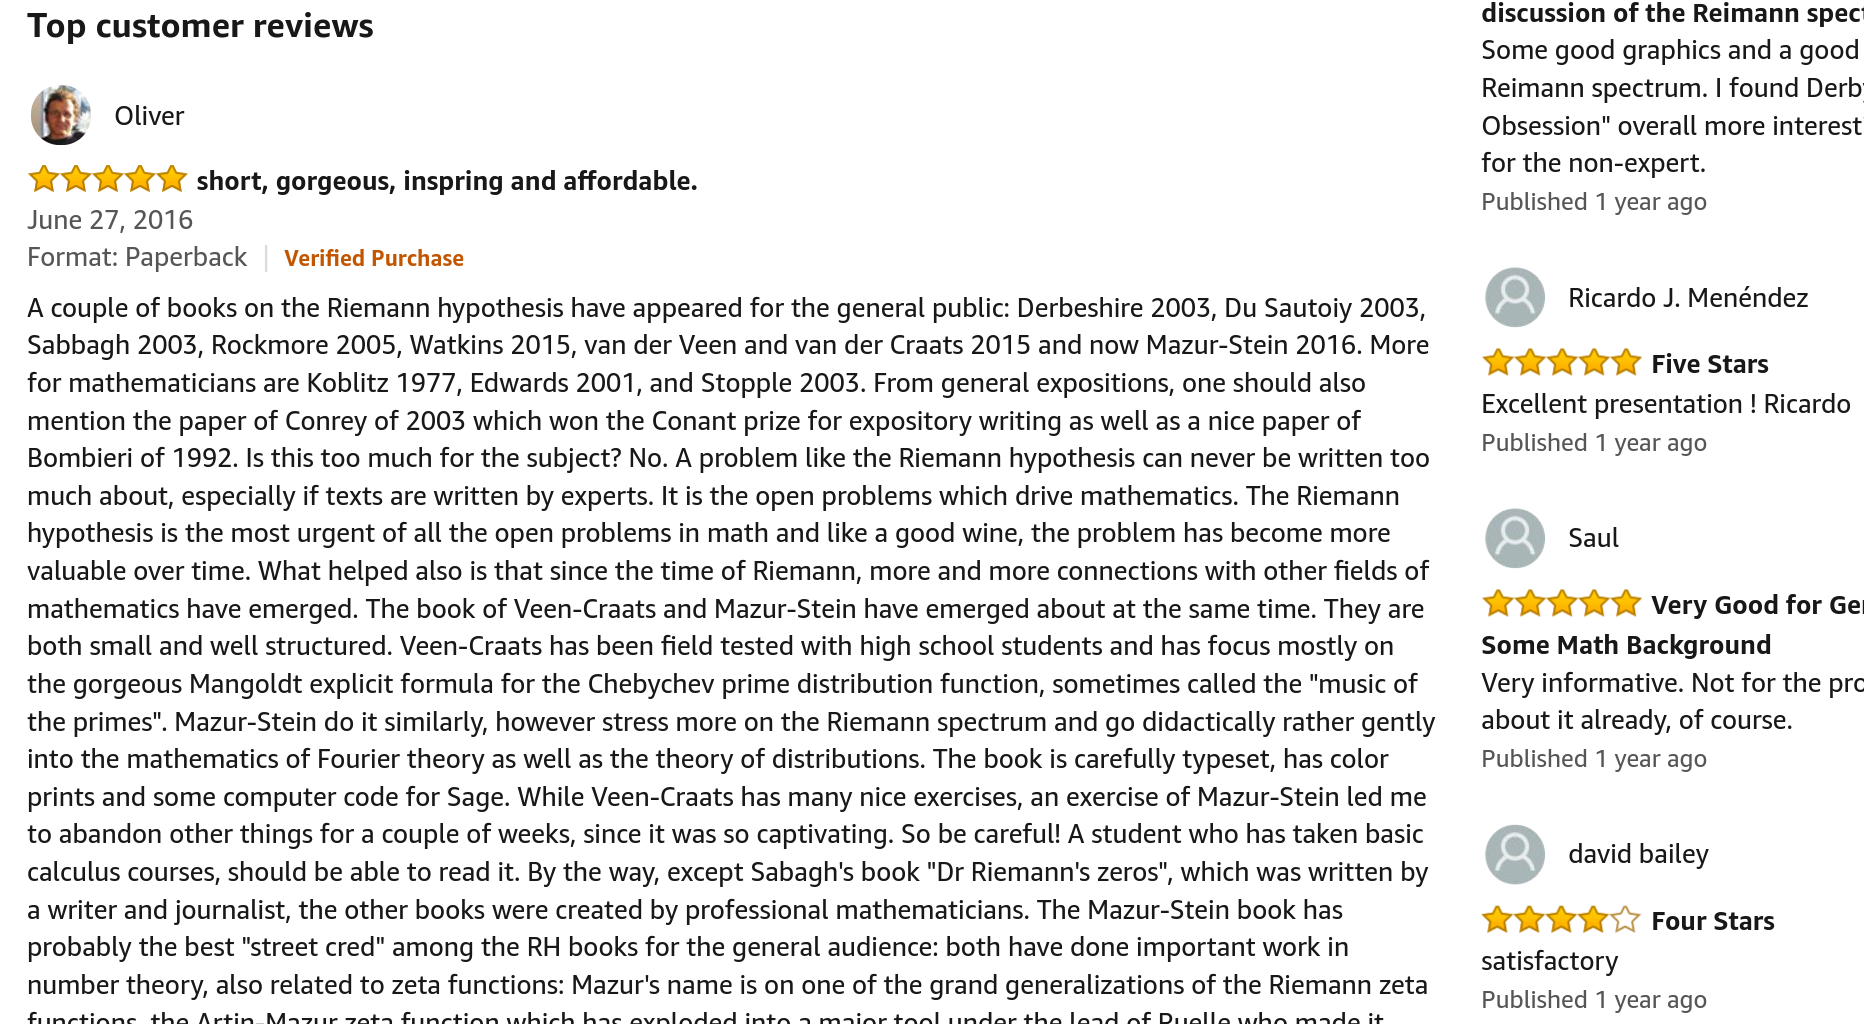
\includegraphics[width=.98\textwidth]{pics/amazon-review.png}

  \vfill

  Negative reviews  due to \textit{production issues}, both with the physical book
  and the Kindle edition....

\end{frame}

\begin{frame}{Reception by Readers}
  \begin{itemize}
    \item Feedback
    \item Sarnak's review in Bulletins
    \item Other reviews
    \item Prizes
  \end{itemize}
\end{frame}

\begin{frame}{Royalties}

  We sold some copies, so Cambridge University Press sent us some money.
  I bought a puppy named Bella!

  \begin{center}
    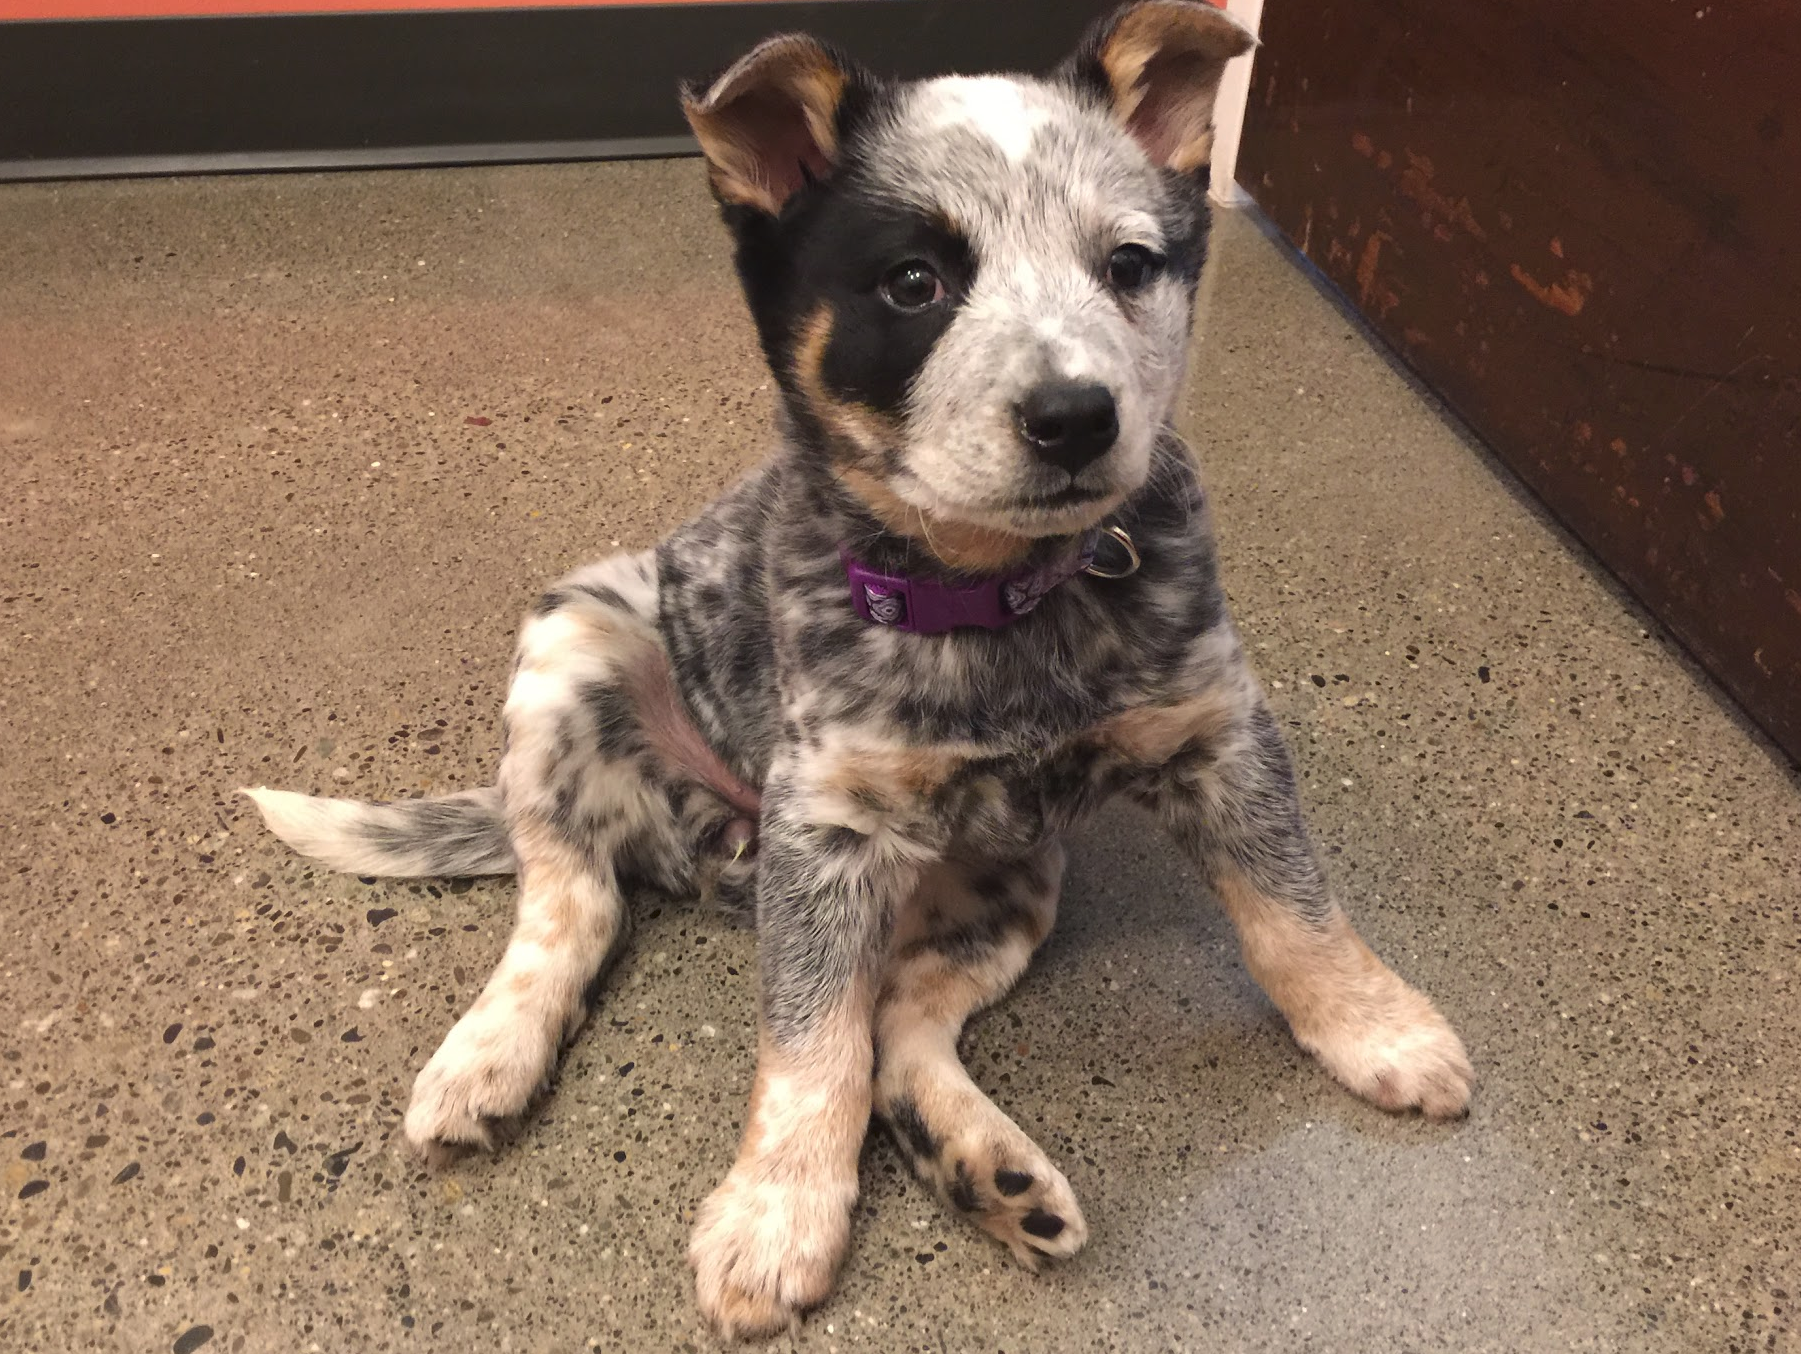
\includegraphics[height=.7\textheight]{pics/bella-puppy.png}
  \end{center}


\end{frame}


\begin{frame}[fragile]
  \frametitle{Translation: what to expect?}
  \begin{verbatim}
Dear Professor Stein,

Prime Numbers and the Riemann Hypothesis

I am delighted to inform you that we are currently
concluding an agreement with Nippon Hyoron Sha for
a Japanese language edition of your book. They plan
to print an edition of 2,500 copies initially, which
will be sold at approximately 2,200 JPY per copy.
  \end{verbatim}

  What to expect?
  \begin{itemize}
    \item  Also Korean?
    \item  Will they bother with French, etc.?
  \end{itemize}
\end{frame}


\begin{frame}
  \frametitle{Future Plans}
  \begin{itemize}
    \item Online fully interactive version.
    \item Related research on $L$-series of elliptic curves, etc.
  \end{itemize}
\end{frame}


\end{document}